%%
%% Meta: Diagramme Lesen
%%

\input{bmsLayoutPage}

\renewcommand{\metaHeaderLine}{Arbeitsblatt}
\renewcommand{\arbeitsblattTitel}{Diagramme Lesen (V 0.1)}

%%%%%%%%%%%%%%%%%%%%%%%%%%%%%%%%%%%%%%%%%%%%%%%%%%%%%%%%%%%%%%%%%%

%\usepackage{amssymb} 
%\usepackage{cancel}

%\newcommand\Ccancel[2][black]{\renewcommand\CancelColor{\color{#1}}\cancel{#2}}


\begin{document}%%
\arbeitsblattHeader{}

\section{Kennzahlen aus Diagrammen lesen}
Lesen Sie, falls möglich, die geforderten Informationen aus den
Diagrammen heraus und berechnen Sie \textbf{falls möglich} die gewünschten Kennzahlen.

\begin{tabular}{c|c}
A: & B: \\
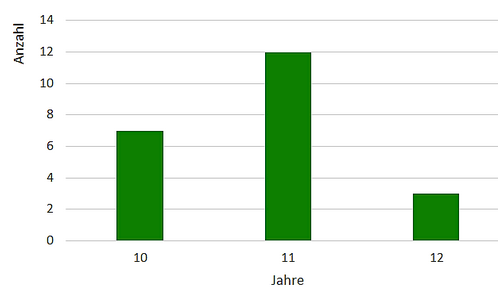
\includegraphics[width=70mm]{img/Grafik_A_Saeulendiagramm.png} &
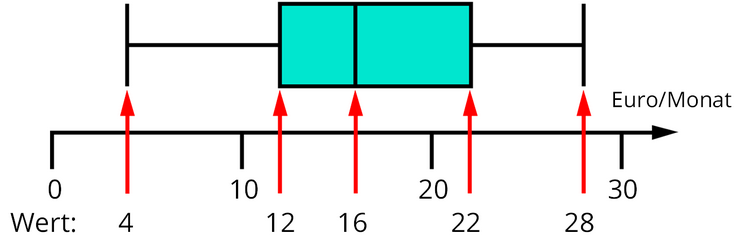
\includegraphics[width=70mm]{img/Grafik_B_Boxplot}\\
\hline
C: & D: \\
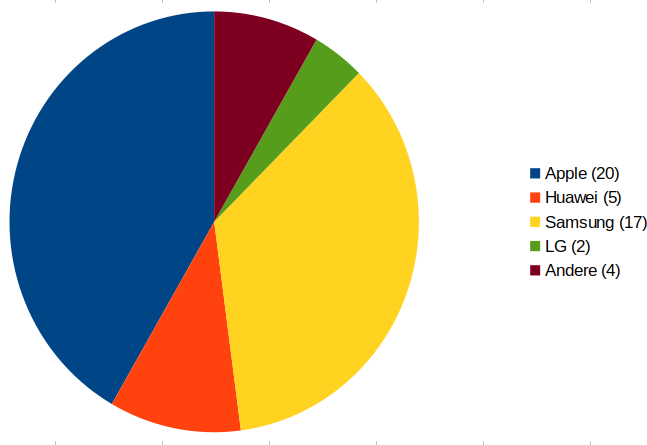
\includegraphics[width=70mm]{img/Grafik_C_Kreisdiagramm.png} &
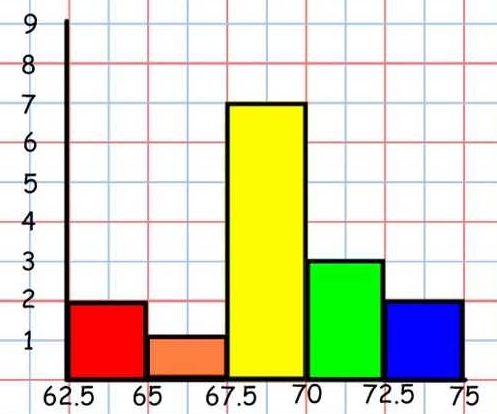
\includegraphics[width=70mm]{img/Grafik_D_Histogramm.png}
\end{tabular}


a) Um welche Art von Diagramm handelt es sich?
   (Auswahl: Balkendiagramm/Säulendiagramm, Kreisdiagramm, Boxplot, Histogramm)

A) \TRAINER{Balkendiagramm/Säulendiagramm}

B) \TRAINER{Boxplot}

C) \TRAINER{Kreisdiagramm}

D) \TRAINER{Histogramm}

\vspace{15mm}
\hrule

b) Handelt es sich um
nominale, ordinale oder kardinale (Intervalle/Verhältnisse) Daten?

A) \TRAINER{Ordinale oder diskretisierte kardinale}

B) \TRAINER{Kardinale}

C) \TRAINER{Nominale}

D) \TRAINER{Kardinale}


\vspace{15mm}
\hrule

c) Bestimmen Sie falls jeweils den Stichprobenumfang $n$:

A) \TRAINER{22}

B) \TRAINER{kann nicht bestimmt werden}

C) \TRAINER{48}

D) \TRAINER{15}


\vspace{15mm}
\hrule

d) Bestimmen Sie jeweils das Minimum:

A) \TRAINER{10}

B) \TRAINER{4}

C) \TRAINER{Es sind nur nominale Daten. Ein Minimum gibt es erst bei
ordinalen Daten.}

D) \TRAINER{Sind nur kategorisierte Daten. Das Minimum zu bestimmen
ist somit unmöglich.}


\vspace{15mm}
\hrule

e) Bestimmen Sie den Mittelwert

A) \TRAINER{$10.\overline{81}$}

B) \TRAINER{nicht möglich, da klassierte Daten}

C) \TRAINER{nicht möglich, da nominale Daten nicht einmal geordnet
werden können.}

D) \TRAINER{Nicht möglich, da klassierte Daten. Wir wissen nicht wo
innerhalb der Säulen sich die Werte befinden.}


\vspace{15mm}
\hrule

f) Bestimmen Sie den Modus:

A) \TRAINER{11}

B) \TRAINER{nicht möglich}

C) \TRAINER{Apple}

D) \TRAINER{nicht möglich}



\vspace{15mm}
\hrule

g) Bestimmen Sie den Median:

A) \TRAINER{11}

B) \TRAINER{16}

C) \TRAINER{nicht möglich, da nur nominale Daten}

D) \TRAINER{nicht möglich, da klassifizierte Daten}

\newpage

h) Bestimmen Sie die Standardabweichung


A) \TRAINER{$\sigma=0.649220766,   S=0.664498639$}

B) \TRAINER{nicht möglich, da Boxplots immer klassifizierte Daten
angeben}

C) \TRAINER{nicht möglich für nominale Daten}

D) \TRAINER{nicht möglich für klassifizierte Daten}


\vspace{15mm}
\hrule


i) Bestimmen Sie die Quartilsdifferenz QD (= Interquartile Range IQR):

A) \TRAINER{1 (= 11-10)}

B) \TRAINER{10}

C) \TRAINER{nicht möglich für nominale Daten}

D) \TRAINER{nicht möglich für klassierte Daten}




\end{document}
